\documentclass{article}
% Change "article" to "report" to get rid of page number on title page
\usepackage{amsmath,amsfonts,amsthm,amssymb}
\usepackage{setspace}
\usepackage{Tabbing}
\usepackage{fancyhdr}
\usepackage{lastpage}
\usepackage{extramarks}
\usepackage{url}
\usepackage{chngpage}
\usepackage{longtable}
\usepackage{soul,color}
\usepackage{graphicx,float,wrapfig}
\usepackage{enumitem}
\usepackage{morefloats}
\usepackage{multirow}
\usepackage{multicol}
\usepackage{indentfirst}
\usepackage{lscape}
\usepackage{pdflscape}
\usepackage{float}
\restylefloat{table}
\usepackage{algorithm}
\usepackage{algorithmic}
%\usepackage{natbib}
\usepackage[toc,page]{appendix}
%\providecommand{\e}[1]{\ensuremath{\times 10^{#1} \times}}

% In case you need to adjust margins:
\topmargin=-0.45in      % used for overleaf
%\topmargin=0.25in      % used for mac
\evensidemargin=0in     %
\oddsidemargin=0in      %
\textwidth=6.5in        %
%\textheight=9.75in       % used for mac
\textheight=9.25in       % used for overleaf
\headsep=0.25in         %

% Homework Specific Information
\newcommand{\hmwkTitle}{Progress Report 1}
\newcommand{\hmwkDueDate}{Monday,\ September\  24,\ 2018}
\newcommand{\hmwkClass}{Final Project}
\newcommand{\hmwkClassTime}{CSE 597}
\newcommand{\hmwkAuthorName}{Sahithi\ Rampalli}
\newcommand{\hmwkNames}{svr46}

% Setup the header and footer
\pagestyle{fancy}
\lhead{\hmwkNames}
\rhead{\hmwkClassTime: \hmwkTitle} 
\cfoot{Page\ \thepage\ of\ \pageref{LastPage}}
\renewcommand\headrulewidth{0.4pt}
\renewcommand\footrulewidth{0.4pt}

%%%%%%%%%%%%%%%%%%%%%%%%%%%%%%%%%%%%%%%%%%%%%%%%%%%%%%%%%%%%%
% Make title

\title{\vspace{2in}\textmd{\textbf{\hmwkClass:\ \hmwkTitle}} \\
\vspace{0.1in}\large{ \hmwkClassTime}\vspace{3in}}

\author{\textbf{\hmwkAuthorName} \\ \vspace{0.1in}
\hmwkDueDate }
\date{} % to take away today's date

%%%%%%%%%%%%%%%%%%%%%%%%%%%%%%%%%%%%%%%%%%%%%%%%%%%%%%%%%%%%%

\begin{document}
\begin{spacing}{1.1}
\maketitle

\newpage
\section*{Abstract}

The purpose of this project is to learn and build an optimized iterative solver for the discrete Poisson Equation on caretesian grid.
I chose to use Cholesky decomposition ($LDL^T$ fatorization) as direct method and Conjugate Gradient as iterative method to solve {Ax=b}.
The results of this project will be used for our research work where we implemented conjugate gradient solver for the same problem on FPGA architecture \cite{FPGACG}. The aim is to compare the performance of the solver on different architectures including CPU and FPGA.
\section{Problem of Interest}

Finite difference numerical method is used to discretize the 2-dimensional poisson equation. On an m{x}n grid, it takes the form
\[(\nabla^2	u)_{ij} = \dfrac{1}{dx^2}(u_{i+1,j} + u_{i-1,j} + u_{i,j+1} + u_{i,j-1} - 4u_{i,j} ) \] 
	Discrete Poisson equation arises in various fields of study such as heat flow, electrostatics, gravity, computational fluid dynamics and many more. The size of the grids on which the equation is applied can go as large as 10s or 100s of 1000s. For such large matrix sizes, it is clearly essential to parallelize and optimize the solvers.
	For direct solver methods, banded LU (a special case of Gaussian Elimination) is the optimal method as the matrix in this problem is diagonal matrix. Further optimization can be done by using $LDL^T$ factorization.
	Since the matrix sizes are really large, direct solvers are usually not preferred as $A^-1$ computation or back filling will be quite expensive. Iterative methods like  Jacobi, SOR, Conjugate Gradients are used to solve discrete Poisson Equation \cite{Berkley1996} . Iterative methods use the idea of nearest-neighbour computing to solve the equation. Methods like FFT and Multigrid can be faster than the iterative methods as they forward the information to points on the grid which are farther than the nearest neighbours. FFTs and multigrid are more specialized to solve problems like poisson, unlike direct solvers like LU decomposition which is used to solve almost any linear system (nonsingular). \cite{FFTPoisson}

\subsection{Numerical Set-up}

\subsubsection{Direct Solver}
	I obtained the $A$ matrix for $LDL^T$ factorization using the matlab command "gallery('poisson', $n$)" where $n$ is the compute grid dimension which is half of the matrix dimension (say $N$). The vector $b$ is populated with random numbers. The same vector is used for both the solvers.

\subsubsection{Iterative Solver}
	For iterative solver, the matrix $A$ is not stored, but every matrix operation is visualized as a stencil operation computed on a grid of dimension $n$ which is half of the matrix dimension ($N$). The vector $b$ is same as that for direct solver.
\\
\newline
The matrix sizes considered for testing are $64x64$, $256x256$ and $1024x1024$. The matrix dimensions for production problem can go upto 10s and 100s of 1000s. For our research work on FPGA, we used maximum matrix size of $10816x10816$.


\section{Solvers}

\subsection{Direct Solver}

As mentioned in the previous section, I use $LDL^T$ factorization as a direct solver for solving discrete poisson equation on large compute grids. An example of the poisson problem is shown in the figure \ref{poisson}.

\begin{center}
	\begin{figure}[H]
	\centering
       \includegraphics[scale=.40]{poisson.png}
        \caption{\label{poisson} Discrete Poisson Problem on 4x4 grid \cite{Berkley1996}.} 
	\end{figure}
\end{center}

Clearly the matrix can be viewed as a symmetric, banded matrix. When a matrix is symmetric, Cholesky decomposition ($LL^T$ factorization) is the optimal way to solve the linear system of equations. Since the above matrix is not only symmetric, but also diagonal dominated, a different version of Cholesky, $LDL^T$ factorization, is the best choice. 
If a matrix $A\epsilon R^{nxn}$ is symmetric and the principal submatrix $A(1:k,1:k)$ is nonsingular for $k=1:n-1$, then there exists a unit lower matrix $L$ and a diagonal matrix $D$ such that $LDL^T$ and the factorization is unique. \cite{MatComp}

The algorithm for $LDL^T$ factorization is shown in listing \eqref{algoLDL}. Here the matrix $A$ is overwritten with $D_i$ for $i=j$ and $L_{ij}$ for $i>j$.
\begin{algorithm}[H]

%\begin{multicols}{2}
\begin{algorithmic}[1]
%\caption{function [A, x, b] = LDLt(A, b)}

%\label{alg:seq}
\FOR{$j=1:n$}
\FOR{$i=1:j-1$ until convergence}
\STATE $v(i) = A(j,i)*A(i,i)$ 
\ENDFOR
\STATE $A(j,j) = A(j,j) - A(j,1:j-1).v(1:j-1)$
\STATE $A(j+1:n,j) = (A(j+1:n, j) - A(j+1:n,1:j-1).v(1:j-1))/A(j,j) $ 
%\STATE $resVec = [resVec, norm(A * x - b)]$ 
%\STATE $j \gets j + 1$	
\ENDFOR
%\STATE $its = j$
\end{algorithmic}
%\end{multicols}
\caption{\label{algoLDL} function [A, x, b] = stdCG(A, b)} 
\end{algorithm}

The algorithm $LDL^T$ factorization requires about $n^3/3$ flops which is almost half the number of flops required for Gaussian Elimination. 

The implementation is also made memory-efficient by writing back to the matrix $A$ and vector $b$ and not using any other extra space. I also made an attempt to store $A$ as a banded matrix to reduce the space further. However, the logic did not work perfectly. I shall work on the logic and update the code in the coming days.

\subsubsection*{Timing and Memory}
For test problem, the chosen sizes of matrix A are $64x64$, $256x256$, $1024x1024$. The production problem size can be as large as $10861x10861$. 
The execution times for different test sizes upon using the G++ compiler optimization flag -O2 is shown in Table \ref{exec_direct}. The flag O2 has been used to optimize on the execution time.
The memory required is measured in terms of number of elements required to be stored for the ease of understanding. The number of elements in Table \ref{exec_direct} is for the matrix $A$ and vector $b$. 

\begin{table}[H]
\begin{center}
%\resizebox{\columnwidth}{!}{%
 \begin{tabular}{| c | c | c |} 
 \hline
$N$ & $Exec time (microseconds)$  & $Number of Elements$  \\ %[0.3ex] 
 \hline
64 & 758 & 4160\\ %\hline
256 &  18680 & 65792\\ %\hline 
1024 &  1151817 & 1049600 \\ %[0.3ex]
 \hline
\end{tabular}%
%}
\end{center}
\caption{\label{exec_direct} The execution time and number of elements stored for different test problem sizes.  } 
\end{table}

The execution time for back filling is shown in Table \ref{backfill_direct}.

\begin{table}[H]
\begin{center}
%\resizebox{\columnwidth}{!}{%
 \begin{tabular}{| c | c |} 
 \hline
$N$ & $Exec time (microseconds)$ \\ %[0.3ex] 
 \hline
64 & 74  \\ %\hline
256 &  372 \\ %\hline 
1024 &  10503  \\ %[0.3ex]
 \hline
\end{tabular}%
%}
\end{center}
\caption{\label{backfill_direct} The execution time for back filling for different test sizes.  } 
\end{table}

We can see that apart from the time for decomposition, the backfilling also takes considerable number of FLOPs and hence execution time. 

The projection of execution time for production problem size $10816$x$10816$ is expected to be of the order of $10^8$. The projection of memory for production problem size $10816$x$10816$ in terms of the number of elements required to be stored is 116996672. Thus the space required grows exponentially with the problem size.


\subsection{Iterative Solver}

I use Conjugate Gradient (CG) method as an iterative solver for solving discrete poisson equation. One reason for choosing conjugate gradient is that it was developed for symmetric and positive definite matrices which is the case in the chosen problem. Also, as we are testing conjugate gradient on FPGA architecture, it would be useful to use this method and test it on CPU to compare the performance of our hardware design for CG with that on CPU.

Convergence criteria: I have chosen the tolerance to be of the order of $10^{-4}$ as this should be sufficient for applications involving discrete poisson equation. My inequality to test for convergence is:
\[ delta = dotProduct(residual_values); \epsilon = 0.0001 \]
\[ log_{10}(\sqrt{|delta|}) >= log_{10}(\epsilon) \]


\begin{algorithm}[H]

%\begin{multicols}{2}
\begin{algorithmic}[1]
%\caption{function [A, x, b] = CG(A, b)}

%\label{alg:seq}
\STATE $n = \text{size}(A,1)$ 
\STATE $x = \text{zeros}(n,1)$
%\STATE $resVec = [\hspace{1mm}]$
\STATE $r_{\text{old}} = b$ ; $p = r_{\text{old}}$ ; $j = 1$
\FOR{$i=1$ until convergence}
\STATE $z = A*p$ 
\STATE ${\alpha} = (r_{\text{old}}, r_{\text{old}})/(z, p)$
\STATE $x = x + \alpha * p$ 
\STATE $r = r_{old} - \alpha * z$
\STATE $\beta = (r, r) \, / \, (r_{\text{old}}, r_{\text{old}})$
\STATE $p = r + \beta* p$;
\STATE $r_{\text{old}} = r$
%\STATE $resVec = [resVec, norm(A * x - b)]$ 
%\STATE $j \gets j + 1$	
\ENDFOR
%\STATE $its = j$
\end{algorithmic}
%\end{multicols}
\caption{\label{algoCG} function [A, x, b] = stdCG(A, b)} 
\end{algorithm}

The Conjugate Gradient algorithm shown in \eqref{algoCG} has a matrix-vector multiplication operation $z=A*p$. However, one can view this operation as a stencil operation applied on the vector $p$. The stencil will be:
\begin{tabular}{|c|c|c|}
\hline
0 & -1 & 0\\ \hline
-1 & 4 & -1 \\ \hline
0 & -1 & 0 \\ \hline
\end{tabular}

This can be very easily deduced from the discrete poisson form shown in section 1.
Applying the stencil operation reduces the number of FLOPs exponentially as the stencil is computed on vector $p$ which is square root times the size of matrix $A$.
Performing $z=A*p$ as a stencil operation is not only compute-efficient but also memory-efficient as we do not have to store matrix $A$.

The convergence plot of $Log_{10}(Residual Values)$ Vs. $iterations$ is shown in the figure \ref{convPlot}.
\begin{center}
	\begin{figure}[H]
	\centering
       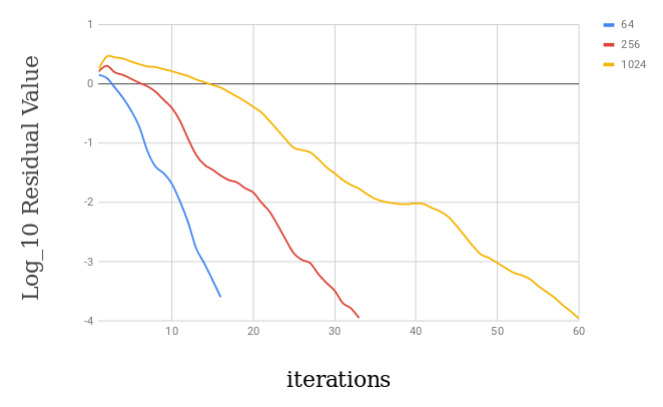
\includegraphics[scale=.40]{convergence.png}
        \caption{\label{convPlot} Convergence Plot} 
	\end{figure}
\end{center}


\subsubsection*{Timing and Memory}
For test problem, the chosen sizes of matrix $A$ are $64x64$, $256x256$, $1024x1024$. The production problem size can be as large as $10861x10861$. 
The execution times for different test sizes upon using the G++ compiler optimization flag -O2 is shown in Table \ref{exec_iter}. The flag O2 has been used to optimize on the execution time.

I have tested the problem for different initializations for vector $x$. Any random initialization (tested multiple times) gives the same set of residual values and number of iterations. The possible reason is that the residual vector $r$ in conjugate gradient method is not much dependent on the values of $x$, which is evident from algorithm \eqref{algoCG}.

\begin{table}[H]
\begin{center}
%\resizebox{\columnwidth}{!}{%
 \begin{tabular}{| c | c|c|c|} 
 \hline
$N$ & $ExecTime (microseconds)$ & $Number of Elements$  \\ %[0.3ex] 
 \hline
64 & 155 & 5*64\\ %\hline
256 &  440 & 5*256\\ %\hline 
1024 &  4988 & 5*1024\\ %[0.3ex]
 \hline
\end{tabular}%
%}
\end{center}
\caption{\label{exec_iter} The execution time and number of elements stored for different test problem sizes.  } 
\end{table}

The size of the vector $b$ required for the problem increases linearly with the problem size.

\section{Solver Comparison}

The table \ref{speedup} shows the speedup of the Conjugate Gradient method over the direct solver. Clearly, conjugate gradient method outperforms direct solver as the number of computations has reduced exponentially. Also, the speedup increases with increase in the matrix size.

From storage point of view, iterative solver wins over direct solver as the matrix $A$ is not stored in the former case (sparse matrix-vector multiplication operation is replaced by stencil operation). The number of elements required for CG increases linearly with problem size unlike the direct method where the growth is exponential.

Even for a production scale problem where matrix size is of the order $10^4$ and more, conjugate gradient will have greater speedup when compared to $LDL^T$ factorization.

\begin{table}[H]
\begin{center}
%\resizebox{\columnwidth}{!}{%
 \begin{tabular}{| c | c |} 
 \hline
$N$ & $Exec time (microseconds)$  \\ %[0.3ex] 
 \hline
64 & 4.8x \\ %\hline
256 & 42.5x \\ %\hline 
1024 &  231x \\ %[0.3ex]
 \hline
\end{tabular}%
%}
\end{center}
\caption{\label{speedup} The speedup of CG over $LDL^T factorization$  } 
\end{table}

\section{Discussion and Conclusions}

From the results it can be concluded that iterative solvers are much better in terms of execution time and memory required than the direct solvers for solving discrete Poisson Equation.

From parallelization perspective, Conjugate Gradient is easier to implement in this case as it mostly involves point-wise operations like dot product, vector addition and one stencil operation. The Direct method involves Matrix vector product. Hence, the matrix has to be carefully decomposed. From performance and space complexity point of view, Conjugate gradient will again outperform due to the exponentially smaller vectors stored in contrast to the matrix in direct method.

\newpage
\begin{appendices}

\section{Acknowledgements}

I would like to acknowledge my advisor at IIIT-Hyderabad, India for guiding me to work on conjugate gradient solver for poisson equation on different architectures. I would like to acknowledge my class mates, Chirag Satish and Amatur Rahman, for helping me fix some implementation errors and clarifying some doubts regarding compute nodes on ACI.

\section{Code}

The code is available of GitHub and can be obtained by cloning:
git clone https://github.com/sahithi-rv/ProjectReport1.git

The instructions for compiling and executing to reproduce the results are mentioned in the READme.md file available in the repository. The file descriptions are also mentioned in the READme.md file.

The compute node used was the node with Intel Broadwell processor (comp-bc-0239).

\section{Licensing and Publishing}
	
	The code published is a free software.
	The licensing information is also available on the git repository page.

\end{appendices}

\bibliographystyle{acm}
\bibliography{main}

\end{spacing}

\end{document}

%%%%%%%%%%%%%%%%%%%%%%%%%%%%%%%%%%%%%%%%%%%%%%%%%%%%%%%%%%%%%}}
